\begin{figure}[H]
   \centering
   % Fila 1: el grafo y el archivo, centrados verticalmente
   \begin{minipage}[c]{0.40\textwidth}
      \centering
      \resizebox{0.78\linewidth}{!}{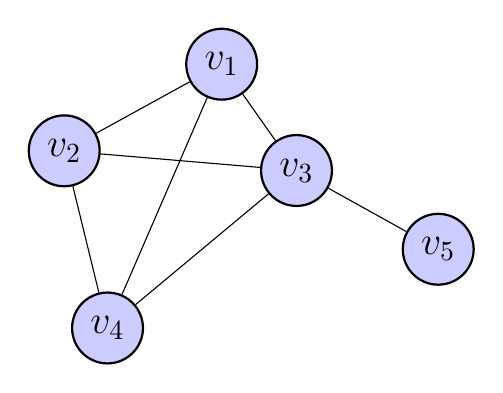
\begin{tikzpicture}[
  scale=1,
  vnode/.style={circle, fill=blue!20, draw=black, thick, minimum size=9mm, inner sep=0pt, font=\Large}
]
  % Vértices
  \node[vnode] (v1) at (2.0, 3.35) {$v_1$};
  \node[vnode] (v2) at (0.0, 2.25) {$v_2$};
  \node[vnode] (v3) at (2.95, 2.0) {$v_3$};
  \node[vnode] (v4) at (0.55, 0.0) {$v_4$};
  \node[vnode] (v5) at (4.75, 1.0) {$v_5$};

  % Aristas
  \foreach \from/\to in {v1/v2, v1/v3, v1/v4, v2/v3, v2/v4, v3/v4, v3/v5}
    \draw (\from) -- (\to);
\end{tikzpicture}
}
   \end{minipage}%
   \hspace{1.5em}%
   \begin{minipage}[c]{0.42\textwidth}
\begin{lstlisting}[framexrightmargin=-4.4pt]
5
0  1  1  1  0
1  0  1  1  0
1  1  0  1  1
1  1  1  0  0
0  0  1  0  0
\end{lstlisting}
   \end{minipage}

   % Fila 2: los pies, alineados arriba y centrados
   \captionsetup{format=plain, justification=centering}
   \begin{minipage}[t]{0.40\textwidth}
      \captionof{figure}{Grafo $G_1$}
      \label{fig:G_1}
   \end{minipage}%
   \hspace{1.5em}%
   \begin{minipage}[t]{0.42\textwidth}
      \captionof{lstlisting}{Archivo \texttt{1\_Mat\_Ady.txt} para guardar la información de $G_1$}
      \label{cod:1_Mat_Ady}
   \end{minipage}
\end{figure}
